\section{Cosmology}
\begin{sectionauthor}
    Sanah Bhimani (Yale University) \\
    Ava Polzin (The University of Chicago) \\
    Dr. Luna Zagorac (Perimeter Institute)
\end{sectionauthor}


\subsection{Theory}

The role of cosmology is to answer ``big-picture" questions about the entirety of the Universe: how and when did it start, what's its shape, how has it been evolving up to today, and what are its contents. In that way it is similar to definitions of ``cosmology" in social sciences and humanities: it is another way we make sense of the Universe around us and how it came to be. Plenty of cosmologists dig into details and smaller questions or certain epochs of the Universe, but for this section we'll take a zoomed-out approach to review our best current understanding of its content, history, and beginning. 

\subsubsection{The Contents of the Universe}

Cosmological observations and experiments tell us at the Universe is expanding, and at an accelerating rate at that. The reason it's expanding has to do with its contents, which are essentially pushing the horizon of the Universe farther and farther away with time. Every single thing described in this guide is found within the Universe, but cosmologists really only divide them into a few types of ``thing:" radiation, matter, and a mysterious ``cosmological constant."

Radiation refers for the most part to light, but can also include very light particles travelling close to the speed of light (like neutrinos). Astronomers spend a lot of time thinking about radiation in the Universe, because a lot of observations are done with light. However, it turns out light is a really tiny budget of the total energy density of the Universe---only about 0.8\%. Most of that budget is the Cosmic Microwave Background (CMB)---the oldest light in the Universe---and cosmologists often don't even include it when doing calculations because it contributes so little. 

Matter is more bulky: it refers to things that have mass and aren't moving close to the speed of light, and makes up about 30\% of the energy density of the Universe. This includes things like planets, stars, galaxies, gasses and dust between them, and more. All of these are examples of ``regular" or ``baryonic" matter, meaning that it's made up of atoms and particles we're familiar with. Then there's dark matter: we know it's dark (meaning, it doesn't interact with light; ``invisible" might have been a better name) and we know that it's matter (meaning, it has mass). We also believe that it's ``cold"---which is cosmologist speak for ``slow-moving"---but we don't know the details. We also know that of the 30\% of matter that exists in the Universe, about 25\% is dark matter and only around 5\% is baryonic matter. As described in the section of galaxies, dark matter is also really important to understanding how galaxies like ours form, making it one of the big mysteries of astronomy and physics today. 

Finally, there is something called a ``cosmological constant." If this sounds uninformative, that's because we know even less about it than dark matter. It doesn't behave like radiation or matter; rather, it seems to be somehow a part of empty space. Each cubic meter of dark matter in the Universe contains the same amount of the cosmological constant, and the more the Universe expands---the more cosmological constant there is. Around 70\% of the energy density of the Universe is in the cosmological constant, which is sometimes also called dark energy or $\Lambda$ (the Greek letter Lambda). This is another huge open question of modern astrophysics. 

Despite not knowing the details of either dark matter or dark energy/$\Lambda$, the big picture view we do know allows us to describe observations of the Universe really well. This is why the ``standard" or ``concordance" model of cosmology is often called $\Lambda$CDM (referring to $\Lambda$, the cosmological constant and cold dark matter -- CDM -- as a generic description of dark matter).   

One ``component" not discussed here is not a component at all, but the shape or curvature of the Universe; nevertheless, curvature sometimes gets added into cosmological equations. Our best data says that we live in a ``flat" Universe, which essentially means that the sum total of all components add up to 100\%. If they added up to more or less than that, we would have reason to believe our Universe is curved, and its cosmology would be very different!

\subsubsection{The History of the Universe}

The picture of the Universe presented in the previous section is valid today; that is to say, $\Lambda$ wasn't always the dominant component in the Universe, and radiation wasn't always such an afterthought. As the Universe expands, its contents get diluted, like pouring water into juice. Its contents dilute at different rates and as a function of redshift $z$, or alternatively the scale factor $a = \frac{1}{1 + z}$; consequently, this dilution is called ``redshifting." Radiation redshifts the fastest, such that its density evolves as $\rho_{\rm{r}} \propto a^{-4}$; this is because there are three spatial dimensions and also the wavelength of the radiation lengthens. Matter is slower: it only redshifts in three dimensions, so $\rho_{\rm{m}} \propto a^{-3}$. The cosmological constant $\Lambda$ doesn't redshift at all; as the name suggests it remains constant, so $\rho_{\rm{\Lambda}} = \rm{const}$.

Knowing this, it's not a surprise that our Universe today is made up mostly of dark energy, some matter, and little radiation: the last two got redshifted away as the Universe evolved, and will continue to do so as it evolves forward. From now until forever, the Universe will expand faster and faster, until all the galaxies grow very distant, the stars run out of gas, and the cosmos grows cold and dark. This scenario is known as the Big Freeze or Heat Death of the Universe, and of several explanations that cosmologists have proposed over the years, our current model favors this one. Thus, the Universe will one day end (a long, long, long time from now): not with a bang, but with a whimper. 



Instead of looking on towards the Universe's eventual doom, cosmologists can instead evolve our Universe backwards in time to understand its past. Looking back to higher redshifts doesn't impact the components of our Universe, but it does impact their relative contributions to the total density of the Universe. For instance, at a redshift of about 0.3 or 3.5 billion years ago, the Universe was made up of equal parts matter and dark energy, with some small contribution from radiation (but not as small as today). To find when matter and radiation were present in equal measure, we have to wind the clock even farther back:
\begin{itemize}
    \item farther back than when the first galaxies formed, when the Universe was about 400 million years old...
    \item farther back than the formation of the first stars, when the Universe was around 200 million years of age...
    \item even farther back than the cosmic microwave background, which was released when the Universe was 300 \textit{thousand} years old... 
\end{itemize}
We have to wind the clock back all the way to the Universe's 50,000$^{\rm{th}}$ birthday: the blink of an eye for a Universe that is approaching 14 billion years of age at the time you're reading this text! Still, important moments in our Universe happened even earlier: for instance, the first nuclei of helium and hydrogen formed about 3 minutes after the Universe was born, and the first neutrons, protons, and electrons---only around a microsecond after its birth.  

\begin{figure}[h!]
    \centering
    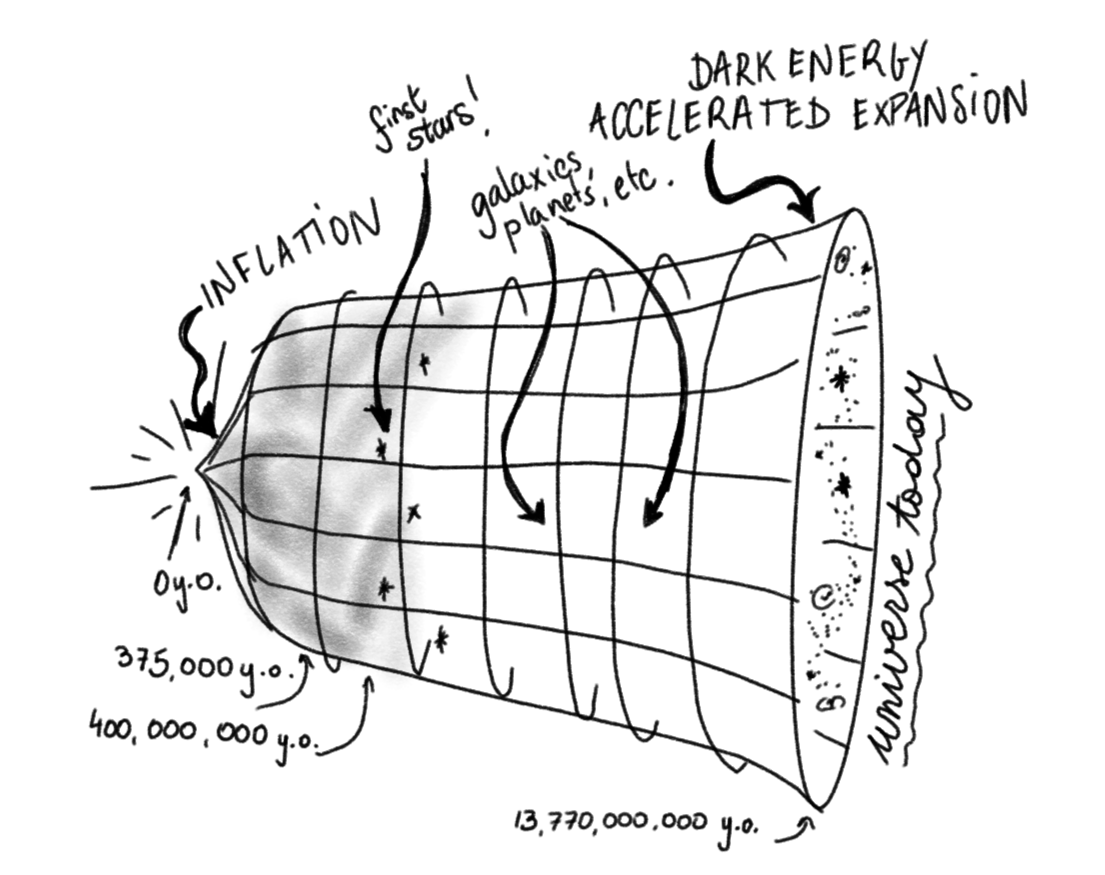
\includegraphics[width=0.6\linewidth]{img/cosmology.png}
    \caption{Starting from today and looking back in time, cosmology can help us trace the size and shape of the Universe as well as its contents, all the way back to its (still mysterious) beginnings.}
    \label{fig:cosmology}
\end{figure}


\subsubsection{The Origin of the Universe}

Now that we have an idea of what happened mere microseconds after the birth of our Universe, a natural question to ask is what came before and how it all started. If we continue turning back the clock until the Universe becomes so small it's essentially just one single point---or, in math and physics speak, it reaches a singularity---we reach the event we've come to know as the Big Bang, or the birth of our Universe. What exactly caused our Universe to start expanding and what came before are questions for which nobody has answers right now. 

Some cosmologists believe there must have been a period immediately after the Big Bang---more precisely, around $10^{-32}$ seconds after---when the Universe rapidly expanded from this singularity. This period is called cosmic inflation, and was initially proposed to solve some problems in modern cosmology, such as why our Universe is flat. Imagine slightly inflating a small balloon and drawing a circle on it: the area of the balloon inside the circle will be very curvy to start. Now, if you inflate the balloon way more and look at the same drawn circle, the area inside it will looks pretty flat. Still, other cosmologists think inflation is too weird, and don't think it happened at all. 

All this to say: while there is a general agreement between cosmologists and physicists on referring to the beginning of the Universe as the Big Bang, there is no consensus on how or why it happened, or even what happened immediately after! These are really big and fundamental questions still open for exploration: what do you think happened at the beginning of everything?

\subsection{Experiment}

Thanks to the speed of light acting as a cosmic speed limit, the farther away an object is (on cosmological distances), the farther back we are looking in time. This allows us to look at the universe as it was across different epochs in the 14 Gyr since the Big Bang, which opens doors for us to measure how the universe has evolved over time. (This is the same principle that lets us look at the properties of, say, galaxies over time, except when we discuss cosmology we are thinking about how the physics behaves more globally.)

\subsubsection{21 cm}

One of the most ubiquitous signals in the universe comes from the warm neutral atomic hydrogen, which emits at 21 cm and can be measured by radio telescopes. Because most of this warm HI is connected with large-scale structure (galaxies, galaxy clusters, filaments of the cosmic web, etc.) even at higher redshift, mapping 21 cm emission allows us to map these structures. 

The effective wavelength at which we observe any particular line varies with redshift -- $\lambda_\mathrm{obs} = \lambda_\mathrm{rest}(1 + z)$. Here $\lambda_\mathrm{obs}$ is the observed wavelength, $\lambda_\mathrm{rest}$ is the rest-frame wavelength (or the wavelength at redshift zero), and $z$ is the redshift. This means that we can map a single line (in this case $\lambda_\mathrm{rest} = 21$ cm) at different redshifts by looking at different wavelengths of radiation. At the same time, higher redshift emission is not just more distant, but also corresponds to when the universe was younger (due to the finite speed of light).

As we map the large-scale structure at different redshifts (in different wavelength slices following the equation above), we can actually track the evolution of that structure over time. This, in turn, allows us to understand something called the baryon acoustic oscillation (BAO) scale at different times in cosmic history. Since the BAO scale is a standard ruler (so is well-constrained and comparable at every redshift), we can use it to calibrate our HI mapping to place constraints on the expansion history of the universe!


\begin{figure}[h!]
    \centering
    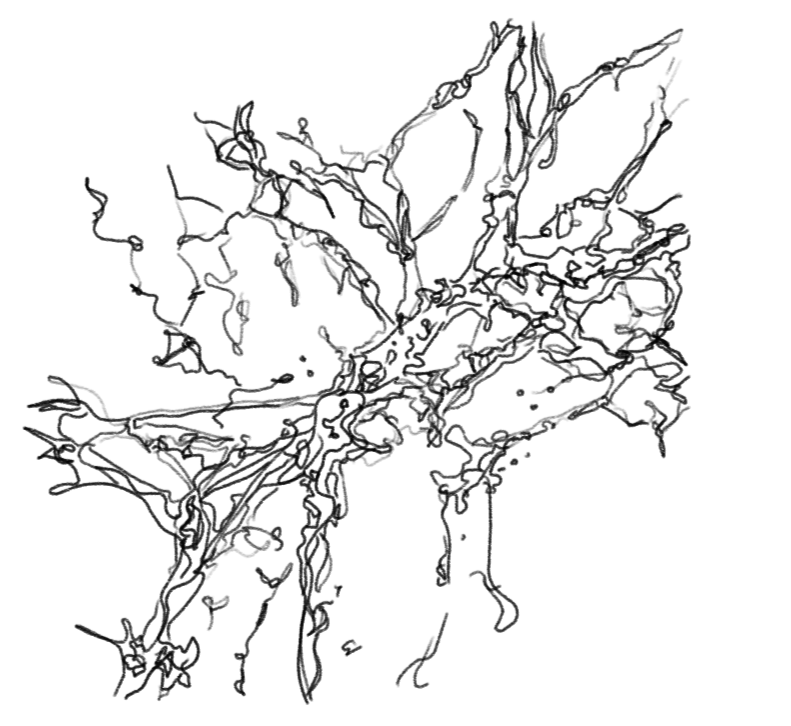
\includegraphics[width=0.5\linewidth]{img/cosmicweb.png}
    \caption{At the largest scales, matter is clustered into \textit{galaxy filaments}, which, as an aggregate, form what we call the \textit{cosmic web}.}
    \label{fig:cosmicweb}
\end{figure}


This expansion history is particularly interesting when dark energy begins to dominate the energy density of the universe at $z \sim 2$. For reference, the first galaxies begin assembling at $z \sim 30$ and the first stars form at $z \sim 15$. With JWST, we've been able to push toward these incredibly high redshifts, so $z \sim 2$ may not seem old, but measurements made at that redshift are of the universe as it was 10 Gyr ago. The Canadian Hydrogen Intensity Mapping Experiment (CHIME) has already detected a cosmological 21 cm signal and is rapidly moving toward being able to recover the BAO scale in their data. It works by mapping the entire Northern sky every night. There is a similar project in the Southern sky, the Hydrogen Intensity Real-time Analysis eXperiment (HIRAX). Other experiments like the Hydrogen Epoch of Reionization Array (HERA) will be able to tell us about the expansion history of the universe at higher redshifts.

\subsubsection{Cosmic Microwave Background}

The Cosmic Microwave Background is remnant radiation from the Big Bang and thus serves as a powerful tool for measuring initial conditions and evolution of the Universe. Measurements of tiny fluctuations in temperature and CMB patterns of light (polarization) have allowed us to extract the age, geometry, and makeup of the Universe, while also providing evidence for dark energy. Future measurements with new, cutting-edge CMB experiments will target their search for inflation, an event predicted to be a rapid, exponential expansion in the very early Universe. Several theories for inflation exist but none have been definitively proven. It's crucial to confirm if inflation occurred because it would provide insight into how small quantum fluctuations in the early, much hotter, and smaller Universe gave rise to the large-scale structures we observe today, like galaxies and galaxy clusters.

We look for inflation in the CMB because, if inflation occured, it would have formed gravitational waves, which would have embedded themselves as a unique signature in our polarization maps of the CMB. If measured, this signal would provide definitive evidence for inflation, eliminate certain inflationary models making it easier to describe the nature of inflation, and provide the only access to physics at Grand Unified Theory (GUT) scales which are inaccessible to particle colliders. Cutting-edge CMB experiments like the Simons Observatory, CMB-S4, BICEP Array will make measurements to detect or constrain the inflationary signal and its energy scale. 

The inflationary signal is extremely faint and this necessitates highly sensitive instrumentation. CMB experiments today are limited by detector count---sensitivity to the CMB, and therefore inflation, can only be achieved with more detectors. The Simons Observatory is currently deploying 4 telescopes with a total of $\sim$60,000 detectors---4$\times$ more than any previous experiment---to the Atacama Desert in Chile. And, CMB-S4, a next-generation experiment will deploy $\sim500,000$ detectors in the 2030s between the South Pole and Chile to measure inflation definitively. 

Increasing the number of detectors allows us to drive down the amount of noise in our data. As we do that, though, ``systematics'' (generally due to the limitations of the instruments/detectors themselves) become the limiting factor in our science results. Since we require precise maps of the CMB to do cosmology, we need to be conscious of these limitations and come up with novel approaches for the mitigation, calibration, and removal of systematic effects, which can be achieved through a combination of hardware and software.

